 \documentclass[answers]{exam}
\newif\ifanswers
\answerstrue % comment out to hide answers

\usepackage{lastpage} % Required to determine the last page for the footer
\usepackage{extramarks} % Required for headers and footers
\usepackage[usenames,dvipsnames]{color} % Required for custom colors
\usepackage{graphicx} % Required to insert images
\usepackage{listings} % Required for insertion of code
\usepackage{courier} % Required for the courier font
\usepackage{lipsum} % Used for inserting dummy 'Lorem ipsum' text into the template
\usepackage{enumerate}
\usepackage{subfigure}
\usepackage{booktabs}
\usepackage{amsmath, amsthm, amssymb}
\usepackage{hyperref}
\usepackage{datetime}
\usepackage{minted}
\settimeformat{ampmtime}
\usepackage{algpseudocode}
\usepackage{algorithmicx}
\usepackage[ruled]{algorithm}
\usepackage{tikz-dependency}
\usepackage{tikz}
\usepackage{changepage}
\usepackage{enumerate}
\usepackage{enumitem}
% \usepackage{bm}
\usetikzlibrary{positioning,patterns,fit,calc}
% Margins
\topmargin=-0.45in
\evensidemargin=0in
\oddsidemargin=0in
\textwidth=6.5in
\textheight=9.0in
\headsep=0.25in

\linespread{1.1} % Line spacing

% Set up the header and footer
%\pagestyle{fancy}
%\rhead{\hmwkAuthorName} % Top left header
%\lhead{\hmwkClass: \hmwkTitle} % Top center head
%\lfoot{\lastxmark} % Bottom left footer
%\cfoot{} % Bottom center footer
%\rfoot{Page\ \thepage\ of\ \protect\pageref{LastPage}} % Bottom right footer
%\renewcommand\headrulewidth{0.4pt} % Size of the header rule
%\renewcommand\footrulewidth{0.4pt} % Size of the footer rule

\pagestyle{headandfoot}
\runningheadrule{}
\firstpageheader{CS 224n}{Assignment 2}{}
\runningheader{CS 224n} {Assignment 2} {Page \thepage\ of \numpages}
\firstpagefooter{}{}{} \runningfooter{}{}{}

\setlength\parindent{0pt} % Removes all indentation from paragraphs

%----------------------------------------------------------------------------------------
%	CODE INCLUSION CONFIGURATION
%----------------------------------------------------------------------------------------

\definecolor{MyDarkGreen}{rgb}{0.0,0.4,0.0} % This is the color used for comments
\definecolor{shadecolor}{gray}{0.9}
\lstloadlanguages{Python} % Load Perl syntax for listings, for a list of other languages supported see: ftp://ftp.tex.ac.uk/tex-archive/macros/latex/contrib/listings/listings.pdf
\lstset{language=Python, % Use Perl in this example
        frame=single, % Single frame around code
        basicstyle=\footnotesize\ttfamily, % Use small true type font
        keywordstyle=[1]\color{Blue}\bf, % Perl functions bold and blue
        keywordstyle=[2]\color{Purple}, % Perl function arguments purple
        keywordstyle=[3]\color{Blue}\underbar, % Custom functions underlined and blue
        identifierstyle=, % Nothing special about identifiers
        commentstyle=\usefont{T1}{pcr}{m}{sl}\color{MyDarkGreen}\small, % Comments small dark green courier font
        stringstyle=\color{Purple}, % Strings are purple
        showstringspaces=false, % Don't put marks in string spaces
        tabsize=5, % 5 spaces per tab
        %
        % Put standard Perl functions not included in the default language here
        morekeywords={rand},
        %
        % Put Perl function parameters here
        morekeywords=[2]{on, off, interp},
        %
        % Put user defined functions here
        morekeywords=[3]{test},
       	%
        morecomment=[l][\color{Blue}]{...}, % Line continuation (...) like blue comment
        numbers=left, % Line numbers on left
        firstnumber=1, % Line numbers start with line 1
        numberstyle=\tiny\color{Blue}, % Line numbers are blue and small
        stepnumber=5 % Line numbers go in steps of 5
}

%----------------------------------------------------------------------------------------
%	NAME AND CLASS SECTION
%----------------------------------------------------------------------------------------

\newcommand{\hmwkTitle}{Word2Vec and Dependency Parsing} % Assignment title
\newcommand{\hmwkClass}{CS\ 224n Assignment \#2} % Course/class
\newcommand{\ifans}[1]{\ifanswers \color{red} \textbf{Solution: } #1 \color{black} \fi}

% \newcommand{\ifans}[1]{}

\input macros.tex
\input std_macros.tex

%----------------------------------------------------------------------------------------
%	TITLE PAGE
%----------------------------------------------------------------------------------------
\qformat{\Large\bfseries\thequestion{}. \thequestiontitle{} (\thepoints{})\hfill}

\title{
\vspace{-1in}
\textmd{\textbf{\hmwkClass:\ \hmwkTitle}}
}
\author{}
%\date{\textit{\small Updated \today\ at \currenttime}} % Insert date here if you want it to appear below your name
\date{}

\setcounter{section}{0} % one-indexing
\begin{document}

\maketitle
\vspace{-3em}

\textbf{Due Date: April 18th, Thursday, 4:30 PM PST.}

In this assignment, you will review the mathematics behind Word2Vec and build a neural dependency parser using PyTorch. For a review of the fundamentals of PyTorch, please check out the PyTorch review session on Canvas. In Part 1, you will explore the partial derivatives involved in training a Word2vec model using the naive softmax loss. In Part 2, you will learn about two general neural network techniques (Adam Optimization and Dropout). In Part 3, you will implement and train a dependency parser using the techniques from Part 2, before analyzing a few erroneous dependency parses.

If you are using LaTeX, you can use \verb!\ifans{}! to type your solutions.

\textbf{Please tag the questions correctly on Gradescope, otherwise the TAs will take points off if you don't tag questions.}
\begin{questions}
    \graphicspath{ {images/} }

% real numbers R symbol
\newcommand{\Real}{\mathbb{R}}

% encoder hidden
\newcommand{\henc}{\bh^{\text{enc}}}
\newcommand{\hencfw}[1]{\overrightarrow{\henc_{#1}}}
\newcommand{\hencbw}[1]{\overleftarrow{\henc_{#1}}}

% encoder cell
\newcommand{\cenc}{\bc^{\text{enc}}}
\newcommand{\cencfw}[1]{\overrightarrow{\cenc_{#1}}}
\newcommand{\cencbw}[1]{\overleftarrow{\cenc_{#1}}}

% decoder hidden
\newcommand{\hdec}{\bh^{\text{dec}}}

% decoder cell
\newcommand{\cdec}{\bc^{\text{dec}}}

\titledquestion{Neural Machine Translation with RNNs}[45]
 In Machine Translation, our goal is to convert a sentence from the \textit{source} language (e.g. Mandarin Chinese) to the \textit{target} language (e.g. English). In this assignment, we will implement a sequence-to-sequence (Seq2Seq) network with attention, to build a Neural Machine Translation (NMT) system. In this section, we describe the \textbf{training procedure} for the proposed NMT system, which uses a Bidirectional LSTM Encoder and a Unidirectional LSTM Decoder.\newline

\begin{figure}[h]
    \begin{center}
        \captionsetup{width=0.8\textwidth}
        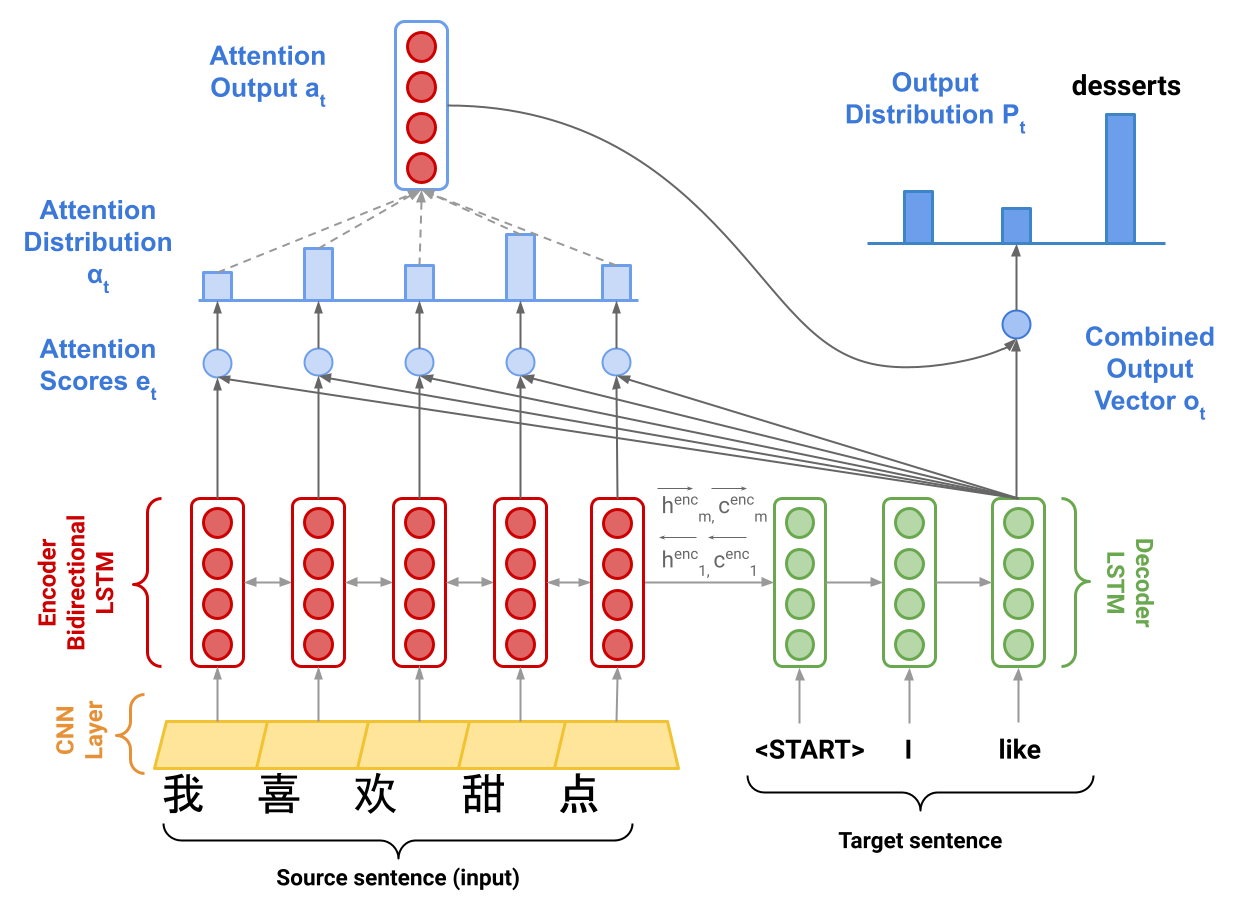
\includegraphics[width=0.8\textwidth]{images/Assignment 4 Figure.png}
        \caption{Seq2Seq Model with Multiplicative Attention, shown on the third step of the decoder. Hidden states $\henc_i$ and cell states $\cenc_i$ are defined on the next page.
        }
        \label{nmt-figure}
    \end{center}
\end{figure}

\subsection*{Model description (training procedure)}
 Given a sentence in the source language, we look up the character or word embeddings from an \textbf{embeddings matrix}, yielding $\bx_1, \dots, \bx_m$ ($\bx_i \in \Real^{e \times 1}$), where $m$ is the length of the source sentence and $e$ is the embedding size. We then feed the embeddings to a \textbf{convolutional layer} \footnote{Checkout \url{https://cs231n.github.io/convolutional-networks} for an in-depth description for convolutional layers if you are not familiar} while maintaining their shapes. We feed the convolutional layer outputs to the \textbf{bidirectional encoder}, yielding hidden states and cell states for both the forwards ($\rightarrow$) and backwards ($\leftarrow$) LSTMs. The forwards and backwards versions are concatenated to give hidden states $\henc_i$ and cell states $\cenc_i$:
 
\begin{align}
    \henc_i = [\hencbw{i}; \hencfw{i}] \enspace &\text{where}\enspace \henc_i \in \Real^{2h \times 1}, \hencbw{i}, \hencfw{i} \in \Real^{h \times 1} &1 \le i \le m \\
    \cenc_i = [\cencbw{i}; \cencfw{i}] \enspace &\text{where} \enspace \cenc_i \in \Real^{2h \times 1}, \cencbw{i}, \cencfw{i} \in \Real^{h \times 1} &1 \le i \le m
\end{align}

We then initialize the \textbf{decoder}'s first hidden state $\hdec_0$ and cell state $\cdec_0$ with a linear projection of the encoder's final hidden state and final cell state.\footnote{If it's not obvious, think about why we regard $[\hencbw{1}, \hencfw{m}]$ as the `final hidden state' of the Encoder.} 

\begin{align}
    \hdec_0 = \bW_{h}[\hencbw{1}; \hencfw{m}] \enspace &\text{where} \enspace \hdec_0 \in \Real^{h \times 1}, \bW_{h} \in \Real^{h \times 2h}\\
    \cdec_0 = \bW_{c}[\cencbw{1}; \cencfw{m}] \enspace &\text{where} \enspace \cdec_0 \in \Real^{h \times 1}, \bW_{c} \in \Real^{h \times 2h}
\end{align}

With the decoder initialized, we must now feed it a target sentence. On the $t^{th}$ step, we look up the embedding for the $t^{th}$ subword,  $\by_t \in \Real^{e \times 1}$. We then concatenate $\by_t$ with the \textit{combined-output vector} $\bo_{t-1} \in \Real^{h \times 1}$ from the previous timestep (we will explain what this is later down this page!\@) to produce $\overline{\by_t} \in \Real^{(e+h) \times 1}$. Note that for the first target subword (i.e. the start token) $\bo_{0}$ is a zero-vector. We then feed $\overline{\by_t}$ as input to the decoder. 

\begin{align}
    \hdec_t, \cdec_t = \text{Decoder}(\overline{\by_t}, \hdec_{t-1}, \cdec_{t-1}) \enspace &\text{where} \enspace \hdec_t \in \Real^{h \times 1}, \cdec_t \in \Real^{h \times 1}\\
\end{align}

We then use $\hdec_t$ to compute  multiplicative attention over $\henc_1, \dots, \henc_m$:

\begin{align}
    \be_{t, i} = (\hdec_t)^T\bW_{\text{attProj}}\henc_i \enspace &\text{where} \enspace \be_{t} \in \Real^{m \times 1}, \bW_{\text{attProj}}\in \Real^{h \times 2h} & 1 \le i \le m \\
    \alpha_t= \text{softmax}(\be_t) \enspace &\text{where} \enspace \alpha_t \in \Real^{m \times 1}\\
    \ba_t = \sum_{i=1}^{m}\alpha_{t,i}\henc_i \enspace &\text{where} \enspace \ba_t \in \Real^{2h \times 1}
\end{align}
 
$\be_{t, i}$ is a scalar, the $i$th element of $\be_{t} \in \Real^{m \times 1}$, computed using the hidden state of the decoder at the $t$th step, $\hdec_t \in \Real^{h \times 1}$, the attention projection $\bW_{\text{attProj}} \in \Real^{h \times 2h}$, and the hidden state of the encoder at the $i$th step, $\henc_i \in \Real^{2h \times 1}$.

We now concatenate the attention output $\ba_t$ with the decoder hidden state $\hdec_t$ and pass this through a linear layer, tanh, and dropout to attain the \textit{combined-output} vector $\bo_{t}$.

\begin{align}   
    \bu_{t} = [\ba_{t}; \hdec_t] \enspace &\text{where} \enspace \bu_t \in  \Real^{3h \times 1} \\
    \bv_t = \bW_{u}\bu_t \enspace &\text{where} \enspace \bv_t \in \Real^{h \times 1}, \bW_{u} \in \Real^{h \times 3h}\\
    \bo_t = \text{dropout}(\text{tanh}(\bv_t)) \enspace &\text{where} \enspace \bo_t \in \Real^{h \times 1}
\end{align}

Then, we produce a probability distribution $\bP_t$ over target subwords at the $t^{th}$ timestep:

\begin{align}
    \bP_t = \text{softmax}(\bW_{\text{vocab}}\bo_{t}) \enspace &\text{where} \enspace \bP_t \in \Real^{V_{t} \times 1}, \bW_{\text{vocab}} \in \Real^{V_{t} \times h}
\end{align}

Here, $V_{t}$ is the size of the target vocabulary. Finally, to train the network we then compute the cross entropy loss between $\bP_t$ and $\bg_{t}$, where $\bg_{t}$ is the one-hot vector of the target subword at timestep $t$:

\begin{align}
    J_t(\theta) = \mathrm{CrossEntropy}(\bP_t,\bg_{t})
\end{align}

Here, $\theta$ represents all the parameters of the model and $J_t(\theta)$ is the loss on step $t$ of the decoder.
Now that we have described the model, let's try implementing it for Mandarin Chinese to English translation!


\subsection*{Setting up Your Local Development Environment}
Ensure that you have \href{https://docs.anaconda.com/free/miniconda/index.html}{conda} installed.
Unzip the starter code, and open the resulting directory in your favorite python integrated development environment (\href{https://code.visualstudio.com/}{Visual Stutio Code} is a popular choice). Open a terminal and navigate (\texttt{cd}) to the directory that contains the \texttt{env-cpu.yml} and \texttt{env-gpu.yml} files. Create and activate the \texttt{cs224n-cpu} conda environment as follows:
\begin{lstlisting}
    conda env create --file env-cpu.yml
    conda activate cs224n-cpu
\end{lstlisting}


\subsection*{Setting up Your Cloud GPU-powered Virtual Machine}
Follow the instructions in the \href{https://docs.google.com/document/d/1FLx0CXIn-SoExxKM1efC-E-6iBjUR4uEnpGnfemMMR0/edit?pli=1#heading=h.4tqnggp12z76}{GCP Guide for CS224n}
(link also provided on website and Ed) to create your VM instance. This should take you approximately 45 minutes. Though you will need the GPU to train your model, we strongly advise that you first develop the code locally and ensure that it runs, before attempting to train it on your VM. GPU time is expensive and limited. It takes approximately \textbf{1.5 to 2 hours} to train the NMT system. We don't want you to accidentally use all your GPU time for debugging your model rather than training and evaluating it. Finally, \textbf{make sure that your VM is turned off whenever you are not using it.}

If your GCP subscription runs out of money, your VM will be temporarily locked and inaccessible. If that happens, please make a private Ed post describing the situation.


After setting up the cloud VM, you should turn it off while you work on the programming assignment locally.

\subsection*{Implementation and written questions}

\begin{parts}
    \part [2] (coding) In order to apply tensor operations, we must ensure that the sentences in a given batch are of the same length. Thus, we must identify the longest sentence in a batch and pad others to be the same length. Implement the \texttt{pad\_sents} function in \texttt{utils.py}, which shall produce these padded sentences.
    
    \part[3] (coding) Implement the \texttt{\_\_init\_\_} function in \texttt{model\_embeddings.py} to initialize the necessary source and target embeddings.

    \part[4] (coding) Implement the \texttt{\_\_init\_\_} function in \texttt{nmt\_model.py} to initialize the necessary model layers (LSTM, CNN, projection, and dropout) for the NMT system.
    
    \part[8] (coding) Implement the \texttt{encode} function in \texttt{nmt\_model.py}. This function converts the padded source sentences into the tensor $\bX$, generates $\henc_1, \dots, \henc_m$, and computes the initial state $\hdec_0$ and initial cell $\cdec_0$ for the Decoder. You can run a non-comprehensive sanity check by executing:
    
\begin{lstlisting}
    python sanity_check.py 1d
\end{lstlisting}
    
    \part[8] (coding) Implement the \texttt{decode} function in \texttt{nmt\_model.py}. This function constructs $\bar{\by}$ and runs the \texttt{step} function over every timestep for the input. You can run a non-comprehensive sanity check by executing:

     
\begin{lstlisting}
    python sanity_check.py 1e
\end{lstlisting}
    
    \part[10] (coding) Implement the \texttt{step} function in \texttt{nmt\_model.py}. This function applies the Decoder's LSTM cell for a single timestep, computing the encoding of the target subword $\hdec_t$, the attention scores $\be_t$, attention distribution $\alpha_t$, the attention output $\ba_{t}$, and finally the combined output $\bo_t$. You can run a non-comprehensive sanity check by executing:
    
    
\begin{lstlisting}
    python sanity_check.py 1f
\end{lstlisting}
           
    
    \part [3] (written) The \texttt{generate\_sent\_masks()} function in \texttt{nmt\_model.py} produces a tensor called \texttt{enc\_masks}. It has shape (batch size, max source sentence length) and contains 1s in positions corresponding to `pad' tokens in the input, and 0s for non-pad tokens. Look at how the masks are used during the attention computation in the \texttt{step()} function (lines 295-296). 
    
    First explain (in around three sentences) what effect the masks have on the entire attention computation.
    Then explain (in one or two sentences) why it is necessary to use the masks in this way.


\end{parts}

Now it's time to get things running! As noted earlier, we recommend that you develop the code on your personal computer.  Confirm that you are running in the proper conda environment and then execute the following command to train the model on your local machine:
    
\begin{lstlisting}
    sh run.sh train_local
    (Windows) run.bat train_local
\end{lstlisting}

To help with monitoring and debugging, the starter code uses tensorboard to log loss and perplexity during training using TensorBoard\footnote{https://pytorch.org/docs/stable/tensorboard.html}. TensorBoard provides tools for logging and visualizing training information from experiments. To open TensorBoard and monitor the training process, run the following in a separate terminal in which you have also activated the \texttt{cs224n-cpu} conda environment, then access tensorboard at \href{http://localhost:6006/}{http://localhost:6006/}.

\begin{lstlisting}
   tensorboard --logdir=runs --port 6006
\end{lstlisting}


\begin{figure}[h]
    \centering
    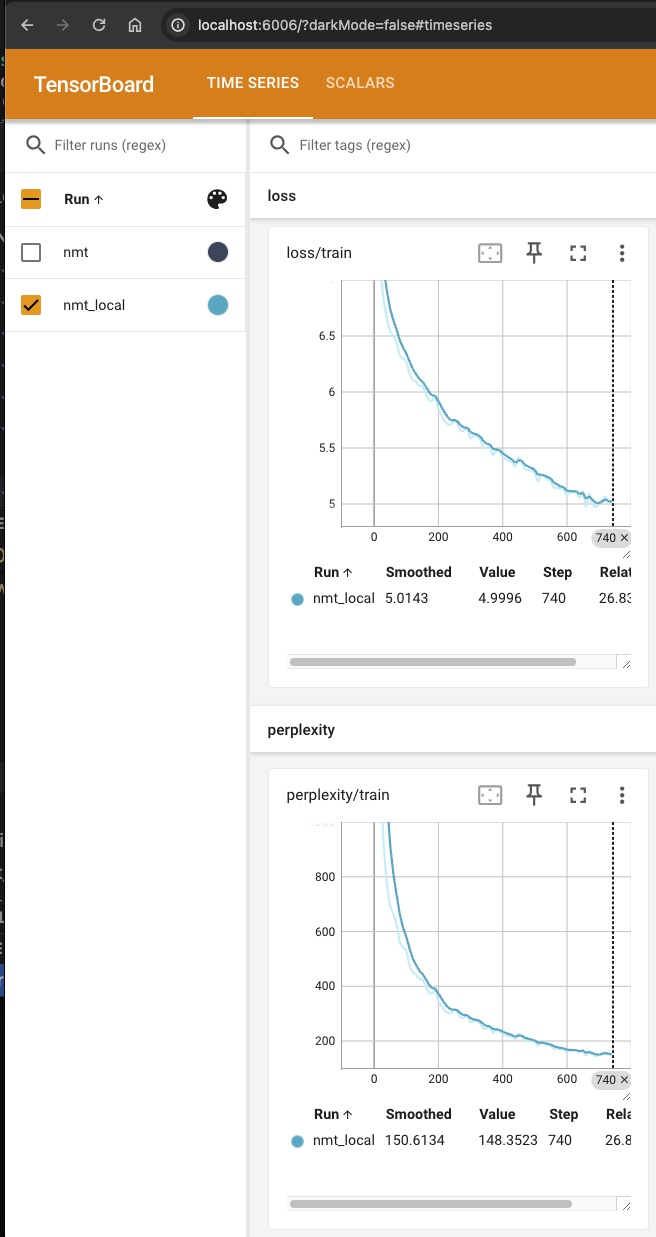
\includegraphics[height=10cm]{images/tensorboard_cpu.jpg}
    \caption{Tensorboard showing loss and perplexity values on your local machine}
    \label{fig:tensorboard-cpu}
\end{figure}

You should see a significant decrease in loss during the initial iterations (Fig \ref{fig:tensorboard-cpu}). Once your code runs for a few hundreds of iterations without crashing, power on your VM from the GCP Console. 

\textbf{Train the NMT system on the VM:} Refer to the GCP How-to Appendix to:
\begin{itemize}
    \item Setup your GCP VM and Obtain SSH Connection Info
    \item Connect to the VM (with SSH Tunneling setup so that you can view remote tensorboard logs)
    \item Copy your code from your computer to the cloud VM
    \item Train the NMT System on the Cloud VM
    \item Download the Gradescope Submission Package from Your Cloud VM
\end{itemize}





\begin{parts}
\setcounter{partno}{7}
\part[3] (written) Once your model is done training (\textbf{this should take under 2 hours on the VM}), execute the following command to test the model:
\begin{lstlisting}
sh run.sh test
\end{lstlisting}
    Please report the model's corpus BLEU Score. It should be larger than 18.
    

    
    \part[4] (written) In class, we learned about dot product attention, multiplicative attention, and additive attention.  As a reminder, dot product attention is $\be_{t,i} = \bs_t^T\bh_i$, multiplicative attention is $\be_{t,i} = \bs_t^T\bW\bh_i$, and additive attention is $\be_{t,i} = \bv^T \text{tanh}(\bW_1\bh_i + \bW_2\bs_t)$.
    
    \begin{subparts}
    \subpart[2] Explain one advantage and one disadvantage of \textit{dot product attention} compared to multiplicative attention.
    \subpart[2] Explain one advantage and one disadvantage of \textit{additive attention} compared to multiplicative attention.
    \end{subparts}
            
    
\end{parts}

    \newpage
    \graphicspath{ {images/} }

\titledquestion{Analyzing NMT Systems}[25]

\begin{parts}

    \part[3] Look at the {\monofam{src.vocab}} file for some examples of phrases and words in the source language vocabulary. When encoding an input Mandarin Chinese sequence into ``pieces'' in the vocabulary, the tokenizer maps the sequence to a series of vocabulary items, each consisting of one or more characters (thanks to the {\monofam{sentencepiece}} tokenizer, we can perform this segmentation even when the original text has no white space). Given this information, how could adding a 1D Convolutional layer after the embedding layer and before passing the embeddings into the bidirectional encoder help our NMT system? \textbf{Hint:} each Mandarin Chinese character is either an entire word or a morpheme in a word. Look up the meanings of 电, 脑, and 电脑 separately for an example. The characters 电 (electricity) and  脑 (brain) when combined into the phrase 电脑 mean computer.


        \textcolor{red}{\textbf{Solution: } Adding a 1D Convolutional layer after the embedding layer can help the NMT system capture local patterns and relationships between characters in the Mandarin Chinese text. Since each character can represent a morpheme or an entire word, the convolutional layer can learn to recognize these patterns and relationships, allowing the model to better understand the meaning of phrases and words. This can lead to improved translation quality, as the model can better capture the semantics of the source language. Additionally, the convolutional layer can help reduce noise in the input by focusing on local features, which can further improve translation accuracy.}


    \part[8] Here we present a series of errors we found in the outputs of our NMT model (which is the same as the one you just trained). For each example of a reference (i.e., `gold') English translation, and NMT (i.e., `model') English translation, please:
    
    \begin{enumerate}
        \item Identify the error in the NMT translation.
        \item Provide possible reason(s) why the model may have made the error (either due to a specific linguistic construct or a specific model limitation).
        \item Describe one possible way we might alter the NMT system to fix the observed error. There are more than one possible fixes for an error. For example, it could be tweaking the size of the hidden layers or changing the attention mechanism.
    \end{enumerate}
    
    Below are the translations that you should analyze as described above. Only analyze the underlined error in each sentence. Rest assured that you don't need to know Mandarin to answer these questions. You just need to know English! If, however, you would like some additional color on the source sentences, feel free to use a resource like \url{https://www.archchinese.com/chinese_english_dictionary.html} to look up words. Feel free to search the training data file to have a better sense of how often certain characters occur.

    \begin{subparts}
        \subpart[2]
        \textbf{Source Sentence:} 贼人其后被警方拘捕及被判处盗窃罪名成立。 \newline
        \textbf{Reference Translation:} \textit{\underline{the culprits were} subsequently arrested and convicted.}\newline
        \textbf{NMT Translation:} \textit{\underline{the culprit was} subsequently arrested and sentenced to theft.}

        \textcolor{red}{\textbf{Solution: } The NMT translation incorrectly uses the singular form "culprit" instead of the plural "culprits". This could be due to the model's inability to correctly identify the plurality of the subject in the source sentence. To fix this, we could increase the size of the training data to include more examples of plural subjects, or we could implement a rule-based post-processing step that checks for subject-verb agreement.}
        

        \subpart[2]
        \textbf{Source Sentence}: 几乎已经没有地方容纳这些人,资源已经用尽。\newline
        \textbf{Reference Translation}: \textit{there is almost no space to accommodate these people, and resources have run out.   }\newline
        \textbf{NMT Translation}: \textit{the resources have been exhausted and \underline{resources have been exhausted}.}
        
        \textcolor{red}{\textbf{Solution: } The NMT translation repeats the phrase "resources have been exhausted" instead of translating the second part of the sentence. This could be due to a limitation in the model's ability to handle complex sentence structures or a lack of training data for similar sentences. To fix this, we could implement a more sophisticated attention mechanism that better captures the relationships between different parts of the sentence, or we could increase the size of the training data to include more examples of complex sentences.}
        

        \subpart[2]
        \textbf{Source Sentence}: 当局已经宣布今天是国殇日。 \newline
        \textbf{Reference Translation}: \textit{authorities have announced \underline{a national mourning today.}}\newline
        \textbf{NMT Translation}: \textit{the administration has announced \underline{today's day.}}
        
        \textcolor{red}{\textbf{Solution: } The NMT translation incorrectly translates "国殇日" as "today's day" instead of "a national mourning today". This could be due to the model's inability to recognize the specific term "国殇日" as a fixed expression. To fix this, we could implement a dictionary-based approach that maps specific terms to their correct translations, or we could increase the size of the training data to include more examples of fixed expressions.}
        
        
        \subpart[2] 
        \textbf{Source Sentence\footnote{This is a Cantonese sentence! The data used in this assignment comes from GALE Phase 3, which is a compilation of news written in simplified Chinese from various sources scraped from the internet along with their translations. For more details, see \url{https://catalog.ldc.upenn.edu/LDC2017T02}. }:} 俗语有云:``唔做唔错"。\newline
        \textbf{Reference Translation:} \textit{\underline{`` act not, err not "}, so a saying goes.}\newline
        \textbf{NMT Translation:} \textit{as the saying goes, \underline{`` it's not wrong. "}}

        \textcolor{red}{\textbf{Solution: } The NMT translation incorrectly translates the Cantonese phrase "唔做唔错" as "it's not wrong" instead of " act not, err not ". This could be due to the model's inability to handle idiomatic expressions or fixed phrases in Cantonese. To fix this, we could implement a rule-based post-processing step that identifies and correctly translates idiomatic expressions, or we could increase the size of the training data to include more examples of idiomatic expressions in Cantonese.}
        
        
    \end{subparts}


    \part[14] BLEU score is the most commonly used automatic evaluation metric for NMT systems. It is usually calculated across the entire test set, but here we will consider BLEU defined for a single example.\footnote{This definition of sentence-level BLEU score matches the \texttt{sentence\_bleu()} function in the \texttt{nltk} Python package. Note that the NLTK function is sensitive to capitalization. In this question, all text is lowercased, so capitalization is irrelevant. \\ \url{http://www.nltk.org/api/nltk.translate.html\#nltk.translate.bleu_score.sentence_bleu}
    } 
    Suppose we have a source sentence $\bs$, a set of $k$ reference translations $\br_1,\dots,\br_k$, and a candidate translation $\bc$. To compute the BLEU score of $\bc$, we first compute the \textit{modified $n$-gram precision} $p_n$ of $\bc$, for each of $n=1,2,3,4$, where $n$ is the $n$ in \href{https://en.wikipedia.org/wiki/N-gram}{n-gram}:
    \begin{align}
        p_n = \frac{ \displaystyle \sum_{\text{ngram} \in \bc} \min \bigg( \max_{i=1,\dots,k} \text{Count}_{\br_i}(\text{ngram}), \enspace \text{Count}_{\bc}(\text{ngram}) \bigg) }{\displaystyle \sum_{\text{ngram}\in \bc} \text{Count}_{\bc}(\text{ngram})}
    \end{align}
     Here, for each of the $n$-grams that appear in the candidate translation $\bc$, we count the maximum number of times it appears in any one reference translation, capped by the number of times it appears in $\bc$ (this is the numerator). We divide this by the number of $n$-grams in $\bc$ (denominator). \newline 

    Next, we compute the \textit{brevity penalty} BP. Let $len(c)$ be the length of $\bc$ and let $len(r)$ be the length of the reference translation that is closest to $len(c)$ (in the case of two equally-close reference translation lengths, choose $len(r)$ as the shorter one). 
    \begin{align}
        BP = 
        \begin{cases}
            1 & \text{if } len(c) \ge len(r) \\
            \exp \big( 1 - \frac{len(r)}{len(c)} \big) & \text{otherwise}
        \end{cases}
    \end{align}
    Lastly, the BLEU score for candidate $\bc$ with respect to $\br_1,\dots,\br_k$ is:
    \begin{align}
        BLEU = BP \times \exp \Big( \sum_{n=1}^4 \lambda_n \log p_n \Big)
    \end{align}
    where $\lambda_1,\lambda_2,\lambda_3,\lambda_4$ are weights that sum to 1. The $\log$ here is natural log.
    \newline
    \begin{subparts}
        \subpart[5] Please consider this example: \newline
        Source Sentence $\bs$: \textbf{需要有充足和可预测的资源。} 
        \newline
        Reference Translation $\br_1$: \textit{resources have to be sufficient and they have to be predictable}
        \newline
        Reference Translation $\br_2$: \textit{adequate and predictable resources are required}
        
        NMT Translation $\bc_1$: there is a need for adequate and predictable resources
        
        NMT Translation $\bc_2$: resources be sufficient and predictable to
        
        Please compute the BLEU scores for $\bc_1$ and $\bc_2$. Let $\lambda_i=0.5$ for $i\in\{1,2\}$ and $\lambda_i=0$ for $i\in\{3,4\}$ (\textbf{this means we ignore 3-grams and 4-grams}, i.e., don't compute $p_3$ or $p_4$). When computing BLEU scores, show your work (i.e., show your computed values for $p_1$, $p_2$, $len(c)$, $len(r)$ and $BP$). Note that the BLEU scores can be expressed between 0 and 1 or between 0 and 100. The code is using the 0 to 100 scale while in this question we are using the \textbf{0 to 1} scale. Please round your responses to 3 decimal places. 

        \ifans{
            \newline
            For $\bc_1$:

            \begin{align*}
            p_1 &= \frac{0 + 0 + 0 + 0 + 0 + 1 + 1 + 1 + 1}{9} = \frac{4}{9} \approx 0.444 \\
            p_2 &= \frac{0 + 0 + 0 + 0 + 0 + 1 + 1 + 1}{8} = \frac{3}{8} \approx 0.375 \\
            len(c) &= 9 \\
            len(r) &= 11 \\
            BP &= \exp(1-\frac{11}{9}) \\
            BLEU &= BP \times \exp\Big(0.5\log(0.444) + 0.5\log(0.375)\Big) \approx 0.327 \\
            \end{align*}

            For $\bc_2$:
            \begin{align*}
            p_1 &= \frac{1 + 1 + 1 + 1 + 1 + 1}{6} = \frac{6}{6} = 1 \\
            p_2 &= \frac{0 + 1 + 1 + 1 + 0}{5} = \frac{3}{5} \approx 0.6 \\
            len(c) &= 6 \\
            len(r) &= 6 \\
            BP &= 1 \\
            BLEU &= BP \times \exp\Big(0.5\log(1) + 0.5\log(0.6)\Big) \approx 0.775
            \end{align*}
        }
        
        Which of the two NMT translations is considered the better translation according to the BLEU Score? Do you agree that it is the better translation?
        
        \ifans{
            \newline
            $\bc_2$ is considered the better translation according to the BLEU Score. However, I think that $bc_1$ is the better translation, as it is more fluent and captures the meaning of the source sentence better.
        }
        
        \subpart[5] Our hard drive was corrupted and we lost Reference Translation $\br_1$. Please recompute BLEU scores for $\bc_1$ and $\bc_2$, this time with respect to $\br_2$ only. Which of the two NMT translations now receives the higher BLEU score? Do you agree that it is the better translation?
        \ifans{
            \newline
            For $\bc_1$:

            \begin{align*}
            p_1 &= \frac{0 + 0 + 0 + 0 + 0 + 1 + 1 + 1 + 1}{9} = \frac{4}{9} \\
            p_2 &= \frac{0 + 0 + 0 + 0 + 0 + 1 + 1 + 1}{8} = \frac{3}{8} \\
            len(c) &= 9 \\
            len(r) &= 6 \\
            BP &= \exp(1-\frac{11}{9}) \\
            BLEU &= 1 \times \exp(0.5 \times \log{\frac{4}{9}} + 0.5 \times \log{\frac{3}{8}}) \approx 0.408
            \end{align*}

            For $\bc_2$:
            \begin{align*}
            p_1 &= \frac{1 + 0 + 0 + 1 + 1 + 0}{6} = \frac{3}{6} \\
            p_2 &= \frac{0 + 0 + 0 + 1 + 0}{5} = \frac{1}{5} \\
            len(c) &= 6 \\
            len(r) &= 6 \\
            BP &= 1 \\
            BLEU &= 1 \times \exp(0.5 \times \log{\frac{3}{6}} + 0.5 \times \log{\frac{1}{5}}) \approx 0.316
            \end{align*}

            Now, $\bc_1$ is considered the better translation according to the BLEU Score, which is reasonalbe as it is more fluent and captures the meaning of the source sentence better.
        }
        
        
        
        \subpart[2] Due to data availability, NMT systems are often evaluated with respect to only a single reference translation. Please explain (in a few sentences) why this may be problematic. In your explanation, discuss how the BLEU score metric assesses the quality of NMT translations when there are multiple reference transitions versus a single reference translation.

        \ifans{
            \newline
            Evaluating NMT systems with respect to only a single reference translation can be problematic because it does not capture the full range of possible translations for a given source sentence. Different reference translations may express the same meaning in different ways, and a single reference translation may not account for all of these variations. When there are multiple reference translations, the BLEU score metric assesses the quality of NMT translations by comparing them to all available references, allowing for a more comprehensive evaluation. In contrast, when there is only a single reference translation, the BLEU score may not accurately reflect the quality of the NMT translation, as it may not capture the full range of possible translations.
        }
        
        \subpart[2] List two advantages and two disadvantages of BLEU, compared to human evaluation, as an evaluation metric for Machine Translation. 
        
        \ifans{
            \newline
            Advantages:
            \begin{enumerate}
                \item BLEU is an automatic evaluation metric, which means it can be computed quickly and easily without the need for human annotators.
                \item BLEU is a widely used metric in the NMT community, which means it allows for easy comparison of different NMT systems and models.
            \end{enumerate}
            
            Disadvantages:
            \begin{enumerate}
                \item BLEU does not capture the full range of possible translations for a given source sentence, as it relies on a limited number of reference translations.
                \item BLEU does not account for the fluency or naturalness of the translation, as it only considers n-gram overlap between the candidate translation and reference translations.
            \end{enumerate}
        }
        
    \end{subparts}


    \part[4] \emph{Beam search} is often employed to improve the quality of machine translation systems. While you were training the model, beam search results for the same example sentence at different iterations were also recorded in TensorBoard, and accessible in the \emph{TEXT} tab (Fig \ref{fig:beam-search-diagnostics-tensorboard}).

    The recorded diagnostic information includes json documents with the following fields: \texttt{example\_source} (the source sentence tokens), \texttt{example\_target} (the ground truth target sentence tokens), and \texttt{hypotheses} (10 hypotheses corresponding to the search result with beam size 10). Note that a predicted translation is often called \emph{hypothesis} in the neural machine translation jargon.

    \begin{subparts}
        \subpart[2] Did the translation quality improve over the training iterations for the model? Give three examples of translations of the example sentence at iterations 200, 3000, and the last iteration to illustrate your answer. For each iteration, pick the first beam search hypothesis as an example:
        
        \ifans{
            \newline
            Yes, the translation quality improved over the training iterations.
            \begin{itemize}
                \item Iteration 800: \textit{I also also noted that the government had been a result of the united nations.}
                \item Iteration 4200: \textit{I have also clarified a number of matters raised by the meeting.}
                \item Last Iteration: \textit{I have also clarified a number of matters raised at the meeting.}
            \end{itemize}
        }
        
        
        \subpart[2] How do various hypotheses resulting from beam search qualitatively compare? Give three other examples of hypotheses proposed by beam search at the last iteration to illustrate your answer.
        
        \ifans{
            \newline
            The hypotheses resulting from beam search qualitatively compare in terms of fluency and accuracy. Some hypotheses are more fluent and natural-sounding, while others may be more literal translations.
            \begin{itemize}
                \item Hypothesis 1: \textit{I have also clarified a number of matters raised at the meeting.}
                \item Hypothesis 2: \textit{Clarification was also given to a number of matters raised at the meeting.}
                \item Hypothesis 3: \textit{I have also clarified a number of matters raised during the meeting".}
            \end{itemize}
        }
        
    \end{subparts}



    \begin{figure}
        \centering
        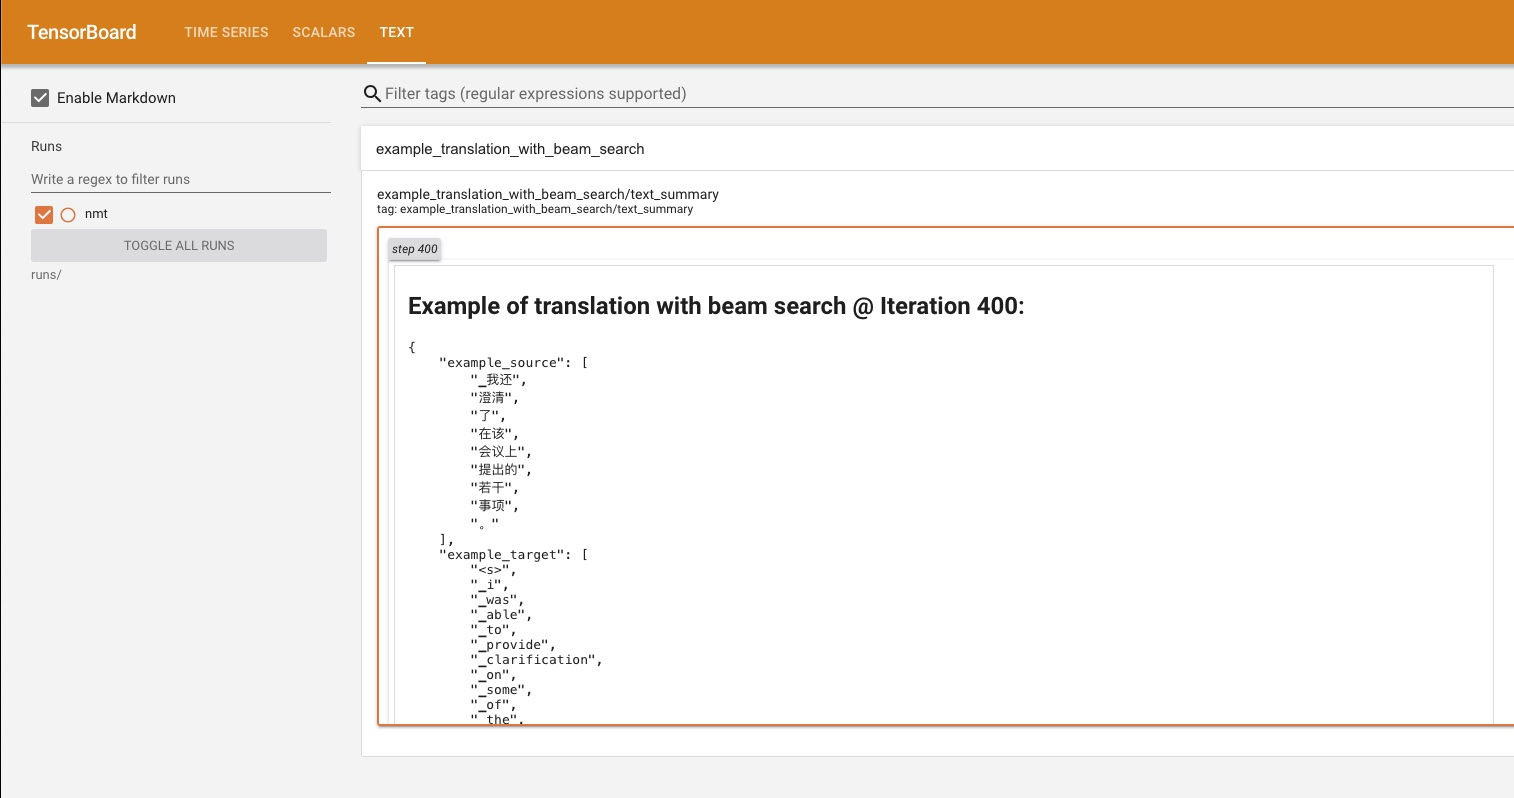
\includegraphics[width=0.7\textwidth]{images/example_translation_beam.jpg}
        \caption{Translation with beam search results for an example sentence are recorded in tensorboard for various iterations. The same data is available in the \texttt{outputs/beam\_search\_diagnostics/} folder in your working directory.}
        \label{fig:beam-search-diagnostics-tensorboard}
    \end{figure}
    

\end{parts}

    \newpage
    \titledquestion{Neural Transition-Based Dependency Parsing}[54]

In this section, you'll be implementing a neural-network based dependency parser with the goal of maximizing performance on the UAS (Unlabeled Attachment Score) metric.\newline

Before you begin, please follow the README to install all the needed dependencies for the assignment. We will be using PyTorch 2.1.2 from \url{https://pytorch.org/get-started/locally/} with the \texttt{CUDA} option set to \texttt{None}, and the tqdm package -- which produces progress bar visualizations throughout your training process. The official PyTorch website is a great resource that includes tutorials for understanding PyTorch's Tensor library and neural networks. \newline

A dependency parser analyzes the grammatical structure of a sentence, establishing relationships between \textit{head} words, and words which modify those heads. There are multiple types of dependency parsers, including transition-based parsers, graph-based parsers, and feature-based parsers. Your implementation will be a {\it transition-based} parser, which incrementally builds up a parse one step at a time. At every step it maintains a \textit{partial parse}, which is represented as follows:
\begin{itemize}
\item A {\it stack} of words that are currently being processed.
\item A {\it buffer} of words yet to be processed.
\item A list of {\it dependencies} predicted by the parser.
\end{itemize}
Initially, the stack only contains ROOT, the dependencies list is empty, and the buffer contains all words of the sentence in order. At each step, the parser applies a {\it transition} to the partial parse until its buffer is empty and the stack size is 1. The following transitions can be applied:
\begin{itemize}
\item \texttt{SHIFT}: removes the first word from the buffer and pushes it onto the stack.
\item \texttt{LEFT-ARC}: marks the second (second most recently added) item on the stack as a dependent of the first item and removes the second item from the stack, adding a \textit{first\_word} $\rightarrow$ \textit{second\_word} dependency to the dependency list.
\item \texttt{RIGHT-ARC}: marks the first (most recently added) item on the stack as a dependent of the second item and removes the first item from the stack, adding a \textit{second\_word} $\rightarrow$ \textit{first\_word} dependency to the dependency list.
\end{itemize}
On each step, your parser will decide among the three transitions using a neural network classifier.

\begin{parts}
    
    \part[4] \textcolor{black}{Go through the sequence of transitions needed for parsing the sentence {\it ``I presented my findings at the NLP conference''}. The dependency tree for the sentence is shown below. At each step, give the configuration of the stack and buffer, as well as what transition was applied this step and what new dependency was added (if any). The first three steps are provided below as an example.} \\

    %\begin{center}
    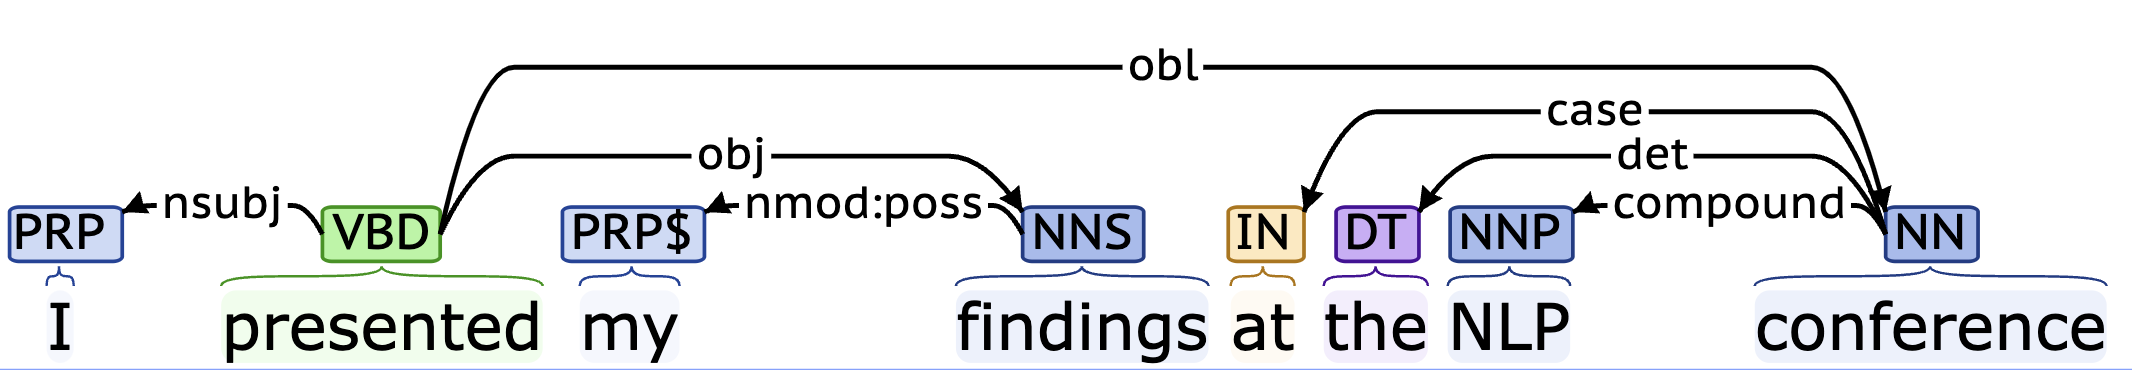
\includegraphics[width=0.8\textwidth]{example.png} \\
    %\end{center}

    \begin{table}[htbp]
    \centering
    \resizebox{1.1\textwidth}{!}{

    \begin{tabular}{ l |l  | l | l}
    Stack & Buffer & New dependency & Transition \\ \hline
    [ROOT] & [I, presented, my, findings, at, the, NLP, conference] &  & Initial Configuration \\
    $[$ROOT, I] & [presented, my, findings, at, the, NLP, conference] &  &  \texttt{SHIFT}  \\
    $[$ROOT, I, presented] & [my, findings, at, the, NLP, conference] &  &  \texttt{SHIFT}  \\
    $[$ROOT, presented] & [my, findings, at, the, NLP, conference] & presented$\to$I &  \texttt{LEFT-ARC}  \\
    $[$ROOT, presented, my] & [findings, at, the, NLP, conference] &  &  \texttt{SHIFT}  \\
    $[$ROOT, presented, my, findings] & [at, the, NLP, conference] &  &  \texttt{SHIFT}  \\
    $[$ROOT, presented, findings] & [at, the, NLP, conference] & findings$\to$my &  \texttt{LEFT-ARC}  \\
    $[$ROOT, presented] & [at, the, NLP, conference] & presented$\to$findings &  \texttt{RIGHT-ARC}  \\
    $[$ROOT, presented, at] & [the, NLP, conference] &  &  \texttt{SHIFT}  \\
    $[$ROOT, presented, at, the] & [NLP, conference] &  &  \texttt{SHIFT}  \\
    $[$ROOT, presented, at, the, NLP] & [conference] &  &  \texttt{SHIFT}  \\
    $[$ROOT, presented, at, the, NLP, conference] & [] &  &  \texttt{SHIFT}  \\
    $[$ROOT, presented, at, the, conference] & [] & conference$\to$NLP &  \texttt{LEFT-ARC}  \\
    $[$ROOT, presented, at, conference] & [] & conference$\to$the &  \texttt{LEFT-ARC}  \\
    $[$ROOT, presented, conference] & [] & conference$\to$at &  \texttt{LEFT-ARC}  \\
    $[$ROOT, presented] & [] & presented$\to$conference &  \texttt{RIGHT-ARC}  \\
    $[$ROOT] & [] & ROOT$\to$presented &  \texttt{RIGHT-ARC} 

    \end{tabular}\newline
    }
    \end{table}
    
    \part[2] A sentence containing $n$ words will be parsed in how many steps (in terms of $n$)? Briefly explain in 1--2 sentences why.
    \ifans{
        \newline
        A sentence containing $n$ words will be parsed in $2n$ steps. This is because the parser will perform $n$ \texttt{SHIFT} operations to move all words from the buffer to the stack, and then it will perform $n$ \texttt{LEFT-ARC} or \texttt{RIGHT-ARC} operations to create dependencies between the words, resulting in a total of $2n$ steps.
    }
       
    
    \part[6] Implement the \texttt{\_\_init\_\_} and \texttt{parse\_step} functions in the \texttt{PartialParse} class in \texttt{parser\_transitions.py}. This implements the transition mechanics your parser will use. You can run basic (non-exhaustive) tests by running \texttt{python parser\_transitions.py part\_c}.

    \part[8] Our network will predict which transition should be applied next to a partial parse. We could use it to parse a single sentence by applying predicted transitions until the parse is complete. However, neural networks run much more efficiently when making predictions about \textit{batches} of data at a time (i.e., predicting the next transition for any different partial parses simultaneously). We can parse sentences in minibatches with the following algorithm. \newline

    \alglanguage{pseudocode}
    \begin{algorithm*}[h]
    \caption{Minibatch Dependency Parsing}
    \begin{algorithmic}
    	\State \textbf{Input:} \texttt{sentences}, a list of sentences to be parsed and \texttt{model}, our model that makes parse decisions
    	%\State
    	%\State Initialize \texttt{partial\_parses} $\to$ []
    	%\For{\textbf{each} sentence \texttt{s} in \texttt{sentences}}
    	%	\State Add a partial parse to \texttt{partial\_parses} with \texttt{stack} = [ROOT], \texttt{buffer} = \texttt{s}, \texttt{dependencies} = []
    	%\EndFor
    	\State
    	\State Initialize \texttt{partial\_parses} as a list of PartialParses, one for each sentence in \texttt{sentences}
    	\State Initialize \texttt{unfinished\_parses} as a shallow copy of \texttt{partial\_parses}
    	%\State
    	\While{\texttt{unfinished\_parses} is not empty}

    		\State Take the first \texttt{batch\_size} parses in \texttt{unfinished\_parses} as a minibatch
    		\State Use the \texttt{model} to predict the next transition for each partial parse in the minibatch
    		\State Perform a parse step on each partial parse in the minibatch with its predicted transition
    		\State Remove the completed (empty buffer and stack of size 1) parses from \texttt{unfinished\_parses}
    	\EndWhile
    	\State
    	\State \textbf{Return:} The \texttt{dependencies} for each (now completed) parse in \texttt{partial\_parses}.
    \end{algorithmic}
    \end{algorithm*}
    
    Implement this algorithm in the \texttt{minibatch\_parse} function in \texttt{parser\_transitions.py}. You can run basic (non-exhaustive) tests by running \texttt{python parser\_transitions.py part\_d}.

    {\it Note: You will need \texttt{minibatch\_parse} to be correctly implemented to evaluate the model you will build in part (e). However, you do not need it to train the model, so you should be able to complete most of part (e) even if \texttt{minibatch\_parse} is not implemented yet.} \newline
    
    \part[20] We are now going to train a neural network to predict, given the state of the stack, buffer, and dependencies, which transition should be applied next.
    
    First, the model extracts a feature vector representing the current state. We will be using the feature set presented in the original neural dependency parsing paper: {\it A Fast and Accurate Dependency Parser using Neural Networks}.\footnote{Chen and Manning, 2014, \url{https://nlp.stanford.edu/pubs/emnlp2014-depparser.pdf}} The function extracting these features has been implemented for you in \texttt{utils/parser\_utils.py}. This feature vector consists of a list of tokens (e.g., the last word in the stack, first word in the buffer, dependent of the second-to-last word in the stack if there is one, etc.). They can be represented as a list of integers $\bw = [w_1, w_2, \dots, w_m]$ where $m$ is the number of features and each $0 \leq w_i < |V|$ is the index of a token in the vocabulary ($|V|$ is the vocabulary size). Then our network looks up an embedding for each word and concatenates them into a single input vector:
    \alns{
    	\bx = [\bE_{w_1}, ..., \bE_{w_m }] \in \mathbb{R}^{dm}
    }
    where $\bE \in \mathbb{R}^{|V| \times d}$ is an embedding matrix with each row $\bE_w$ as the vector for a particular word $w$ with dimension d. We then compute our prediction as:
    \alns{
    	\bh &= \relu(\bx \bW   + \bb_1) \\
    	\bl &= \bh \bU + \bb_2 \\
    	\byt &= \smx(l) \\
    }
    where \bh \space is referred to as the hidden layer, \bl \space is referred to as the logits, $\byt$ \space is referred to as the predictions, and $\relu(z) = \max(z, 0)$). We will train the model to minimize cross-entropy loss:
    \alns{
    	J(\theta) &= CE(\by, \byt) = -\sum \limits_{j = 1}^{3} \by_j \log \byt_j
    } where $\by_j$ denotes the $j$th element of $\by$.
    To compute the loss for the training set, we average this $J(\theta)$ across all training examples.
    
    \begin{enumerate}[label=\roman*.]
    
        \item \textcolor{black}{Compute the derivative of $\bh = \relu(\bx \bW + \bb_1)$ with respect to $\bx$. For simplicity, you only need to show the derivative $\frac{\partial h_i}{\partial x_j}$ for some index $i$ and $j$. You may ignore the case where the derivative is not defined at 0.}
        
        \ifans{
            \newline
            \alns{
                \frac{\partial h_i}{\partial x_j} = 
                \begin{cases}
                    w_{ji} & \text{if } x_j \bW_{ij} + b_{1i} > 0 \\
                    0 & \text{otherwise}
                \end{cases}
            }
        }
        \item \textcolor{black}{Recall in part 1b, we computed the partial derivative of $\bJ_{\text{naive-softmax}}(\bv_c, o, \bU)$. Likewise, please compute the partial derivative of $J(\theta)$ with respect to the $i$th entry of $\bl$, which is denoted as $\bl_i$. Specifically, compute $\frac{\partial CE(\by, \byt)}{\partial \bl_i}$, assuming that $\bl \in \R^3$, $\byt \in \R^3$, $\by \in \R^3$, and the true label is $c$. \\
        \textbf{Hints}: You may recall from part 1a, $\frac{\partial CE(\by, \byt)}{\partial \bl_i} = \sum_j \frac{\partial CE(\by, \byt)}{\partial \byt_j}\frac{\partial \byt_j}{\partial \bl_i}$, and $\frac{\partial CE(\by, \byt)}{\partial \byt_j}=0$ if $j \neq c$. 
        }

        \ifans{
            \newline

            \alns{
                \frac{\partial J}{\partial l_i} &= \left( \frac{\partial J}{\partial \hat{y}_i} \frac{\partial \hat{y}_i}{\partial l_i} \right) + \sum_{j \neq i} \left( \frac{\partial J}{\partial \hat{y}_j} \frac{\partial \hat{y}_j}{\partial l_i} \right) \\
                &= \left(-\frac{y_i}{\hat{y}_i}\right) \left(\hat{y}_i(1 - \hat{y}_i)\right) + \sum_{j \neq i} \left(-\frac{y_j}{\hat{y}_j}\right) \left(-\hat{y}_i \hat{y}_j\right) \\
                &= -y_i(1 - \hat{y}_i) + \sum_{j \neq i} y_j \hat{y}_i \\
                &= -y_i + y_i \hat{y}_i + \hat{y}_i \sum_{j \neq i} y_j \\
                &= -y_i + \hat{y}_i \left(y_i + \sum_{j \neq i} y_j\right) \\
                &= -y_i + \hat{y}_i \left(\sum_{j=1}^{3} y_j\right)
            }
            Since the true label vector $\by$ is one-hot, the sum of its elements is 1.
            $$\frac{\partial J}{\partial l_i} = \hat{y}_i - y_i$$
        }

        \item We will use UAS score as our evaluation metric. UAS refers to Unlabeled Attachment Score, which is computed as the ratio between number of correctly predicted dependencies and the number of total dependencies despite of the relations (our model doesn't predict this).\newline
    
   In \texttt{parser\_model.py} you will find skeleton code to implement this simple neural network using PyTorch. Complete the \texttt{\_\_init\_\_}, \texttt{embedding\_lookup} and \texttt{forward} functions to implement the model. Then complete the \texttt{train\_for\_epoch} and \texttt{train} functions within the \texttt{run.py} file.
   
    Finally execute \texttt{python run.py} to train your model and compute predictions
    on test data from Penn Treebank (annotated with Universal Dependencies). 
    
    \textbf{Note:}
    \begin{itemize}
        \item For this assignment, you are asked to implement Linear layer and Embedding layer. Please \textbf{DO NOT} use \textbf{torch.nn.Linear} or  \textbf{torch.nn.Embedding} module in your code, otherwise you will receive deductions for this problem. 
        \item Please follow the naming requirements in our TODO if there are any, e.g. if there are explicit requirements about variable names you have to follow them in order to receive full credits. You are free to declare other variable names if not explicitly required. 
    \end{itemize}
    
    \textbf{Hints:}
    \begin{itemize}
        \item Each of the variables you are asked to declare (\texttt{self.embed\_to\_hidden\_weight}, \newline \texttt{self.embed\_to\_hidden\_bias}, \texttt{self.hidden\_to\_logits\_weight}, \newline \texttt{self.hidden\_to\_logits\_bias}) corresponds to one of the variables above (\bW, $\bb_1$, \bU, $\bb_2$).  
        \item It may help to work backwards in the algorithm (start from $\byt$) and keep track of the matrix/vector sizes.  
        \item Once you have implemented \texttt{embedding\_lookup (e)} or \texttt{forward (f)} you can call \texttt{python parser\_model.py} with flag \texttt{-e} or \texttt{-f} or both to run sanity checks with each function. These sanity checks are fairly basic and passing them doesn't mean your code is bug free.
        \item
            When debugging, you can add a debug flag: \texttt{python run.py -d}. This will cause the code to run over a small subset of the data, so that training the model won't take as long. Make sure to remove the \texttt{-d} flag to run the full model once you are done debugging.

        \item
            When running with debug mode, you should be able to get a loss smaller than 0.2 and a UAS larger than 65 on the dev set (although in rare cases your results may be lower, there is some randomness when training).
        
        \item It should take up to \textbf{15 minutes} to train the model on the entire training dataset, i.e., when debug mode is disabled.
        
        \item When debug mode is disabled, you should be able to get a loss smaller than 0.08 on the train set and an Unlabeled Attachment Score larger than 87 on the dev set. For comparison, the model in the original neural dependency parsing paper gets 92.5 UAS. If you want, you can tweak the hyperparameters for your model (hidden layer size, hyperparameters for Adam, number of epochs, etc.) to improve the performance (but you are not required to do so).
    \end{itemize}
    
    \textbf{Deliverables:}
        \begin{itemize}
            \item Working implementation of the transition mechanics that the neural dependency parser uses in \texttt{parser\_transitions.py}. 
            \item Working implementation of minibatch dependency parsing in \texttt{parser\_transitions.py}. 
            \item Working implementation of the neural dependency parser in \texttt{parser\_model.py}. (We'll look at and run this code for grading).
            \item Working implementation of the functions for training in \texttt{run.py}. (We'll look at and run this code for grading).
            \item \textbf{Report the best UAS your model achieves on the dev set and the UAS it achieves on the test set in your written submission}.
            
            \ifans{
                \newline
                Best UAS on dev set: 88.56 \\
                UAS on test set: 89.20
            }
    \end{itemize}
    \end{enumerate}
    
    
\part[12] We'd like to look at example dependency parses and understand where parsers like ours might be wrong. For example, in this sentence:

\begin{center}
 {
 \begin{dependency}
 \begin{deptext}
Moscow  \& sent \& troops \& into  \& Afghanistan \& .     \\
 PROPN \& VERB  \& NOUN  \& ADP \& PROPN \& PUNCT \\
 \end{deptext}
 \depedge{2}{1}{nsubj}
 \depedge{2}{3}{dobj}
 \deproot{2}{root}
 \depedge{3}{5}{nmod}
 \depedge{5}{4}{case}
 \depedge[edge unit distance=2.25ex]{2}{6}{punct}
 \end{dependency}
 }
 \end{center}

the dependency of the phrase \emph{into Afghanistan} is wrong, because the phrase should modify \emph{sent} (as in \textit{sent into Afghanistan}) not \emph{troops} (because \textit{troops into Afghanistan} doesn't make sense, unless there are somehow weirdly some troops that stan Afghanistan). Here is the correct parse:

\begin{center}
 {
 \begin{dependency}
 \begin{deptext}
Moscow  \& sent \& troops \& into  \& Afghanistan \& .     \\
 PROPN \& VERB  \& NOUN  \& ADP \& PROPN \& PUNCT \\
 \end{deptext}
 \depedge{2}{1}{nsubj}
 \depedge{2}{3}{dobj}
 \deproot{2}{root}
 \depedge[edge unit distance=2ex]{2}{5}{nmod}
 \depedge{5}{4}{case}
 \depedge[edge unit distance=2.25ex]{2}{6}{punct}
 \end{dependency}
 }
 \end{center}

More generally, here are four types of parsing error:
\begin{itemize}
    \item \textbf{Prepositional Phrase Attachment Error}: In the example above, the phrase \textit{into Afghanistan} is a prepositional phrase\footnote{For examples of prepositional phrases, see: https://www.grammarly.com/blog/prepositional-phrase/}.
    A Prepositional Phrase Attachment Error is when a prepositional phrase is attached to the wrong head word (in this example, \textit{troops} is the wrong head word and \textit{sent} is the correct head word).
    More examples of prepositional phrases include \textit{with a rock}, \textit{before midnight} and \textit{under the carpet}. 
    \item \textbf{Verb Phrase Attachment Error}: In the sentence \textit{Leaving the store unattended, I went outside to watch the parade}, the phrase \textit{leaving the store unattended} is a verb phrase\footnote{For examples of verb phrases, see: https://examples.yourdictionary.com/verb-phrase-examples.html}. 
    A Verb Phrase Attachment Error is when a verb phrase is attached to the wrong head word (in this example, the correct head word is \textit{went}).
    \item \textbf{Modifier Attachment Error}: In the sentence \textit{I am extremely short}, the adverb \textit{extremely} is a modifier of the adjective \textit{short}. A Modifier Attachment Error is when a modifier is attached to the wrong head word (in this example, the correct head word is \textit{short}).
    \item \textbf{Coordination Attachment Error}: In the sentence \textit{Would you like brown rice or garlic naan?}, the phrases \textit{brown rice} and \textit{garlic naan} are both conjuncts and the word \textit{or} is the coordinating conjunction. The second conjunct (here \textit{garlic naan}) should be attached to the first conjunct (here \textit{brown rice}). A Coordination Attachment Error is when the second conjunct is attached to the wrong head word (in this example, the correct head word is \textit{rice}). Other coordinating conjunctions include \textit{and}, \textit{but} and \textit{so}.
\end{itemize}
In this question are four sentences with dependency parses obtained from a parser. Each sentence has one error type, and there is one example of each of the four types above. 
For each sentence, state the type of error, the incorrect dependency, and the correct dependency. While each sentence should have a unique error type, there may be multiple possible correct dependencies for some of the sentences.
To demonstrate: for the example above, you would write: 
\begin{itemize}
    \item \textbf{Error type}: Prepositional Phrase Attachment Error 
    \item \textbf{Incorrect dependency}: troops $\rightarrow$ Afghanistan 
    \item \textbf{Correct dependency}: sent $\rightarrow$ Afghanistan
\end{itemize}

\textit{\textbf{Note}: 
There are lots of details and conventions for dependency annotation. 
If you want to learn more about them, you can look at the UD website: \url{http://universaldependencies.org}\footnote{But note that in the assignment we are actually using UDv1, see: \url{http://universaldependencies.org/docsv1/}} or the short introductory slides at: \url{http://people.cs.georgetown.edu/nschneid/p/UD-for-English.pdf}.
Note that you \textbf{do not} need to know all these details in order to do this question. In each of these cases, we are asking about the attachment of phrases and it should be sufficient to see if they are modifying the correct head.
In particular, you \textbf{do not} need to look at the labels on the the dependency edges -- it suffices to just look at the edges themselves. }

\medskip

i. \\
\begin{center}
{

\begin{dependency}[] 
 \begin{deptext}
The \& university \& blocked \& the \& acquisition \& , \& citing \& concerns \& about \& the \& risks \& involved \& . \\
DET \& NOUN \& VERB \& DET \& NOUN \& PUNCT \& VERB \& NOUN \& ADP \& DET \& NOUN \& VERB \& PUNCT \\
\end{deptext}
\depedge{2}{1}{det}
\depedge{3}{2}{nsubj}
\deproot[edge unit distance=5ex]{3}{root}
\depedge{5}{4}{det}
\depedge{3}{5}{obj}
\depedge{7}{6}{punct}
\depedge{5}{7}{advcl}
\depedge{7}{8}{obj}
\depedge{11}{9}{case}
\depedge{11}{10}{det}
\depedge{8}{11}{nmod}
\depedge{11}{12}{acl}
\depedge[edge unit distance=1.7ex]{3}{13}{punct}
\end{dependency}
 }
\end{center}

\ifans{
    \begin{itemize}
        \item \textbf{Error type}: Verb Phrase Attachment Error
        \item \textbf{Incorrect dependency}: acquisition $\rightarrow$ citing 
        \item \textbf{Correct dependency}: blocked $\rightarrow$ citing
    \end{itemize}
}

%%%%%%%%%%%%%%%%%%%%%%%%%%%%%%%

ii. \\
 \begin{center}
 \color{black}
 {\small
 \begin{dependency}
 \begin{deptext}
 Brian \& has \& been \& one \& of  \& the \& most \& crucial \& elements \& to  \& the \& success \& of  \& Mozilla \& software \& .     \\
 PROPN \& AUX \& AUX  \& NUM \& ADP \& DET \& ADV  \& ADJ     \& NOUN     \& ADP \& DET \& NOUN    \& ADP \& PROPN   \& NOUN \& PUNCT \\
 \end{deptext}
 \depedge{4}{1}{nsubj}
 \depedge{4}{2}{aux}
 \depedge{4}{3}{aux}
 \deproot[edge unit distance=5.5ex]{4}{root}
 \depedge{9}{5}{case}
 \depedge{9}{6}{det}
 \depedge{9}{7}{advmod}
 \depedge{9}{8}{amod}
 \depedge{4}{9}{nmod}
 \depedge{12}{10}{case}
 \depedge{12}{11}{det}
 \depedge{9}{12}{nmod}
 \depedge{15}{13}{case}
 \depedge{15}{14}{compound}
 \depedge{12}{15}{nmod}
 \depedge[edge unit distance=1.65ex]{4}{16}{punct}
 \end{dependency}
 }
 \end{center}


 \ifans{
    \begin{itemize}
        \item \textbf{Error type}: Modifier Attachment Error
        \item \textbf{Incorrect dependency}: elements $\rightarrow$ most
        \item \textbf{Correct dependency}: crutial $\rightarrow$ most
    \end{itemize}
 }
%%%%%%%%%%%%%%%%%%%%%%%%%%%%%%%

\medskip

iii. \\
\begin{center}
 {\small

 \begin{dependency}[] 
 \begin{deptext}
Investment \& Canada \& declined \& to \& comment \& on \& the \& reasons \& for \& the \& goverment \& decision \& . \\
NOUN \& PROPN \& VERB \& PART \& VERB \& ADP \& DET \& NOUN \& ADP \& DET \& NOUN \& NOUN \& PUNCT \\
\end{deptext}
\depedge{2}{1}{compound}
\depedge{3}{2}{nsubj}
\deproot[edge unit distance=5.75ex]{3}{root}
\depedge{5}{4}{mark}
\depedge{3}{5}{xcomp}
\depedge{8}{6}{case}
\depedge{8}{7}{det}
\depedge{5}{8}{obl}
\depedge{12}{9}{case}
\depedge{12}{10}{det}
\depedge{12}{11}{compound}
\depedge[edge unit distance=1.5ex]{3}{12}{nmod}
\depedge[edge unit distance=1.7ex]{3}{13}{punct}
\end{dependency}

 }
 \end{center}

 \ifans{
    \begin{itemize}
        \item \textbf{Error type}: Prepositional Phrase Attachment Error
        \item \textbf{Incorrect dependency}: declined $\rightarrow$ decision
        \item \textbf{Correct dependency}: reasons $\rightarrow$ decision
    \end{itemize}
 }

iv. \\
 \begin{center}
 {\small
 \begin{dependency}[] 
 \begin{deptext}
People \& benefit \& from \& a \& separate \& move \& that \& affects \& three \& US \& car \& plants \& and \& one \& in \& Quebec \\
NOUN \& VERB \& ADP \& DET \& ADJ \& NOUN \& PRON \& VERB \& NUM \& PROPN \& NOUN \& NOUN \& CCONJ \& NUM \& ADP \& PROPN \\
\end{deptext}
\depedge{2}{1}{nsubj}
\deproot[edge unit distance=3ex]{2}{root}
\depedge{6}{3}{case}
\depedge{6}{4}{det}
\depedge{6}{5}{amod}
\depedge{2}{6}{obl}
\depedge{8}{7}{nsubj}
\depedge{6}{8}{acl:relcl}
\depedge{12}{9}{nummod}
\depedge{12}{10}{compound}
\depedge{12}{11}{compound}
\depedge{8}{12}{obj}
\depedge{14}{13}{cc}
\depedge{8}{14}{conj}
\depedge{16}{15}{case}
\depedge{14}{16}{nmod}
\end{dependency}
 }
 \end{center}

    \ifans{
        \begin{itemize}
            \item \textbf{Error type}: Coordination Attachment Error
            \item \textbf{Incorrect dependency}: affects $\rightarrow$ one
            \item \textbf{Correct dependency}: plants $\rightarrow$ one
        \end{itemize}
    }


\part[2] Recall in part (e), the parser uses features which includes words and their part-of-speech (POS) tags. Explain the benefit of using part-of-speech tags as features in the parser?

\ifans{
    \newline
    Part-of-speech tags provide additional syntactic information about the words in a sentence, which can help the parser disambiguate between different meanings of words and improve the accuracy of dependency parsing. For example, knowing that a word is a noun or a verb can help the parser determine its role in the sentence and which other words it should be connected to.
}

\end{parts}

\end{questions}

\Large{\textbf{Submission Instructions}}

\normalsize
You shall submit this assignment on GradeScope as two submissions -- one for ``Assignment 3 [coding]" and another for `Assignment 3 [written]":
\begin{enumerate}
    \item Run the \texttt{collect\_submission.sh} script on the cloud VM to produce your \texttt{assignment3.zip} file. See \emph{How to Download the Gradescope Submission Package from Your Cloud VM} in the GCP How-to Appendix.
    \item Upload your \texttt{assignment3.zip} file to GradeScope to ``Assignment 3 [coding]".
    \item Upload your written solutions to GradeScope to ``Assignment 3 [written]". When you submit your assignment, make sure to tag all the pages for each problem according to Gradescope's submission directions. Points will be deducted if the submission is not correctly tagged.
\end{enumerate}
\end{document}